\section{Angular}
\setauthor{Raffeiner Christine}
\begin{wrapfigure}{r}{0.3\textwidth}
    \begin{center}
      
\includegraphics[width=0.4\textwidth]{pics/Angular_Logo.png}
      \caption{Angular Logo von https://angular.io}
    \end{center}
\end{wrapfigure}
Angular ist ein TypeScript-basiertes, clientseitiges Webapplikations- und JavaScript-Framework 
was bedeutet, dass es für die Entwicklung von Webseiten und Webapplikationen ausgelegt ist. 
Es unterstützt die Verwendung des MVC(Model-View-Controller)-Pattern und vereinfacht die 
Erstellung und das Layoutieren von Single-Page-Applications (SPA) mit TypeScript,
HTML und einer Formatierungssprache. Mögliche Formatierungssprache sind CSS, SCSS SASS und Less.
\newline
\newline
Angular unterscheidet im Prinzip zwischen zwei Arten von Modulen. Zum Einen, das App-Modul, welches das Root-Module beinhaltet und als erstes Modul der Anwendung geladen und initialisiert 
wird und zum Anderen weitere Feature-Module, die sogenannten Components, Services und andere 
notwendige Dateien, die für ein bestimmtes Feature relevant sind.
Durch den Gebrauch des Model-View-Controller-Pattern von Angular wird die Wiederholung 
von Code mithilfe der Erstellung und Wiederverwendbarkeit von Komponenten, die 
statische HTML-Tags mit dynamischen Inhalten verbinden, verhindert.
\newline
\newline
Ein großer Vorteil von Angular ist es, dass es im Gegensatz zu anderen Frameworks über die Funktion 
einer bidirektionalen Verbindung verfügt. Das heißt, dass die Änderung eines 
Wertes einer Variable in einem Textfeld im HTML ebenfalls Auswirkungen auf die Variable im TypeScript 
hat und vice versa. Weitere Vorteile von Angular sind unter anderem, dass Angular ein 
Open Source Framework mit einer MIT Lizenz ist.
\newline
Weiteres stellt Angular umfangreiche Funktionen zur Verfügung, die direkt bereitgestellt sind.
Wie diese Funktionen zu implementieren sind, wird von Angular bereits vorgegeben und erspart somit 
die Überlegung der Implementierung. Zudem werden Zeit und fallweise Kosten gespart, da diese nicht erst
selbst programmiert werden müssen. \cite{noauthor_angular_nodate}, \cite{noauthor_angular_2021}

\subsection{TypeScript}
\begin{wrapfigure}{r}{0.3\textwidth}
    \begin{center}
      
\includegraphics[width=0.4\textwidth]{pics/TS_Logo.png}
      \caption{TypeScript Logo von https://thenewstack.io/how-typescript-helps-enterprise-developers/}
    \end{center}
\end{wrapfigure} 
TypeScript ist eine Programmiersprache, die von Microsoft entwickelt und gewartet wird. 
Sie ist eine streng syntaktische Variante von JavaScript und fügt der Sprache eine optionale 
statische Typisierung hinzu. Es kann zur Entwicklung von JavaScript-Anwendungen sowohl für 
die clientseitige als auch für die serverseitige Ausführung verwendet werden. TypeScript ist für 
die Entwicklung großer Anwendungen konzipiert und lässt sich in JavaScript umwandeln. 
\newline
TypeScript ist keine Programmiersprache für sich allein. Es ist vielmehr eine Kombination aus Werkzeugen und 
optionalen, entfernbaren Typen. TypeScript ermöglicht es einem beliebige 
JavaScript-Tools, -Bibliotheken und -Frameworks zu verwenden.
\newline
TypeScript bezieht sich auf mehrere verschiedene Dinge:
\begin{itemize}
    \item einen Type-Checker für die beiden Sprachen TypeScript und JavaScript
    \item eine übergeordnete Sprache, die die Typensyntax zu JavaScript hinzufügt
    \item den offizielle Compiler, der Code typisiert und umwandelt
\end{itemize}
All diese Komponenten werden benötigt, um JavaScript eine statische Typisierung hinzuzufügen 
und Werkzeuge bereitzustellen, die die Verwendung einfach und komfortabel machen.
\newline
Der TypeScript-Compiler ist selbst in TypeScript geschrieben und zu JavaScript kompiliert. Er ist unter der Apache 
License 2.0 lizenziert. \cite{noauthor_typescript_2022}, \cite{noauthor_softwareentwicklung_nodate}

\subsubsection{JavaScript}
JavaScript (kurz JS) ist leichtgewichtige, interpretierte Skriptsprache. Ihre Bekanntheit hat 
sie hauptsächlich als Skriptsprache für Webseiten erhalten, um Benutzerinteraktionen auszuwerten, 
Inhalte zu verändern, nachzuladen oder zu generieren. JavaScript wird auch außerhalb von Browsern 
angewandt und dient ebenfalls für die Programmierung von Prototypen. Die Sprache bietet 
sowohl objektorientierte, aber klassenlose, imperative als auch deklarative Programmierung an. 
Der Standard für JavaScript ist ECMAScript. \cite{noauthor_javascript_nodate}, \cite{noauthor_javascript_2022}, \cite{noauthor_javascript-grundlagen_nodate}

\subsection{CSS}
\begin{wrapfigure}{r}{0.3\textwidth}
    \begin{center}
      
\includegraphics[width=0.2\textwidth]{pics/CSS_Logo.png}
      \caption{CSS Logo}
    \end{center}
\end{wrapfigure} 
CSS auch Cascading Style Sheets ist eine Formatierungssprache für HTML-, SVG- und XML-Dokumente.
Somit behandelt CSS das Design oder den Stil und nicht den Inhalt von Webseiten. 
Beispielsweise können damit Schriftarten, Farben, Linien, Höhen, Breiten und Positionierung auf einer 
Webseite definieren werden. CSS ermöglicht es ein einmal erstelltes Design schnell und 
einfach in ein anderes Projekt zu übertragen. CSS stellt einen Standard dar und wird vom 
World Wide Web Consortium (W3C) gemanagt und weiterentwickelt. 
\newline
Darüber hinaus wird eine responsive Darstellung von CSS unterstützt. Anders gesagt heißt dass, das mittels CSS 
passende Darstellungsformen für unterschiedliche Geräte angefangen von Monitoren zu Druckern 
bis hin zu Smartphones definiert werden können. Mittels Media Queries können in CSS auch Geräteeigenschaften Breite und Höhe des Browserfensters
ausgelesen werden. Eigenschaften, die bestimmt werden können sind:
\begin{itemize}
    \item Breite und Höhe des Gerätes
    \item Orientierung (Quer- oder Hochformat)
    \item Bildschirmauflösung
\end{itemize}
CSS wird von allen gängigen Browsern 
unterstützt, allerdings kann es zu Einschränkungen bzw. Fehlern bei der Darstellung des Layouts in 
Browsern kommen - übermäßig davon betroffen sind veraltete Browser. \cite{noauthor_css_nodate}, \cite{noauthor_cascading_2022}, \cite{noauthor_css_nodate-1}, \cite{noauthor_css_nodate-2}

\subsubsection{World Wide Web Consortium}
Beim World Wide Web Consortium (W3C) handelt es sich um ein Gremium, dass technische 
Spezifikationen und Richtlinien zur Standardisierung der Techniken im World Wide Web entwickelt.
Andere bekannte Beispiele für Technologien, die durch das W3C standardisierte werden sind, HTML 
SVG und XML. \cite{noauthor_world_nodate}, \cite{noauthor_world_2022}

\subsection{SCSS}
SCSS ist die erweiterte Version von CSS. Es können Variablen definiert werden, die zur Folge haben, dass
der Code verkürzt wird. \cite{noauthor_unterschied_nodate}

\subsection{SASS}
\label{chap:stylesheet}
SASS basiert auf Ruby und heißt ausgeschrieben SassScript. Es steht unter der MIT-Lizenz und gilt daher als Open Source.
SASS bietet im Gegensatz zu CSS zusätzlich die Funktion von: 
\begin{itemize}
    \item Variablen (wie SCSS)
    \item Mathematische Funktionen wie Multiplizieren, Dividieren, Addieren und Subtrahieren (+, -, *, / )
    \item Funktionen
    \item Schleifen
    \item Fallunterscheidungen (wie if und else)
    \item Mixins (Vorlagen, die selbst erstellt oder bei der Verwendung eines Frameworks einfach in den eigenen Code eingebettet werden können)
    \item Vererbung (mittels Selektor)
\end{itemize}
Ein großer Nachteil von SASS ist, dass es zuerst kompiliert werden muss. Das heißt anders als in CSS,
wo Änderungen in der CSS-Datei sofort Auswirkungen auf der Webseite haben, müssen in SASS die Änderungen
erst in CSS übersetzt werden. Im Gegensatz dazu spricht für SASS die freie Auswahl der Syntax. Ob man nun die vorgegebene 
Syntax benutzt oder lieber die gewohnte SCSS- / CSS-Syntax verwendet. \cite{noauthor_sass_nodate}, \cite{noauthor_sass_nodate-2}, \cite{noauthor_grose_nodate}

\subsection{Less}
Genau wie SCSS oder SASS ist Less eine Obermenge von CSS- und somit ebenfalls eine Stylesheet-Sprache.
Vergleichsweise zu SASS ist die Verwendung von Mixins (Vorlagen), Variablen, Berechnungen und Verzweigungen.
Less ist in JavaScript geschrieben und muss ebenfalls kompiliert werden. Allerdings können 
Mithilfe eines Watch-Mode Änderungen automatisch im Webbrowser angezeigt werden. \cite{noauthor_sass_nodate-1}, \cite{noauthor_less_nodate}

\subsection{HTML}
\begin{wrapfigure}{r}{0.3\textwidth}
  \begin{center}
    
\includegraphics[width=0.2\textwidth]{pics/HTML_Logo.png}
    \caption{CSS Logo von https://de.wikipedia.org/wiki/HTML5}
  \end{center}
\end{wrapfigure} 
HTML - ausgeschrieben Hypertext Markup Language - ist eine bekannte textbasierte Auszeichnungssprache für die 
Anzeige und Strukturierung von Webseiten. HTML macht sich sogenannte Tags zu Nutze, um die verschiedensten
Inhalte wie Text, Bilder oder Videos anzuzeigen. Der derzeitige Standard von HTML ist XHTML (Extensible Hypertext Markup Language) und HTML5.
XHTML gehört zu XML, einer Auszeichnungssprache und Dateiformat und erweitert die Auszeichnungssprache HTML.
\newline
HTML5 enthält detaillierte Verarbeitungsmodelle, um mehr kompatible Implementierungen zu fördern: 
Es erweitert, verbessert und vereinfacht das für Dokumente verfügbare Format und führt 
Formatierungs- und Anwendungsprogrammierschnittstellen (APIs) für komplexe Webanwendungen ein. HTML5 ist 
vermehrt für Suchmaschinen optimiert und fördert im Gegensatz zu alten Versionen userorientierte Webseiten.
Zusätzlich zu den Anzeigeelementen verfügt HTML über nicht sichtbare Inhalte namens Metadaten. Diese Daten sind im normalen 
Gebrauch und für User nicht sichtbar. Suchmaschinen allerdings können sie lesen und nicht nur das, sondern auch ihre Suchergebnisse dahingehend
anpassen. Befinden sich keine Metadaten im HTML-Code, versuchen Suchmaschinen sich etwas von der Webseite zusammenzulesen.
HTML-Quellcode kann in jedem Editor geschrieben und von jedem Browser interpretiert werden. \cite{noauthor_hypertext_2022}, \cite{noauthor_html_nodate}, \cite{noauthor_html_nodate-1}

\subsection{NodeJS}
\begin{wrapfigure}{r}{0.3\textwidth}
  \begin{center}
    
\includegraphics[width=0.2\textwidth]{pics/NodeJS_Logo.png}
    \caption{NodeJS Logo von https://de.wikipedia.org/wiki/HTML5}
  \end{center}
\end{wrapfigure}
Node.js ist ein plattformübergreifendes Open-Source Framework, die der MIT-Lizenz unterliegt, und für 
die Entwicklung eigenständiger JavaScript-Programme, Netzwerktools und Webapplikationen verwendet wird.
Der JavaScript-Code kann außerhalb von Webbrowsern laufen und bietet neben Netzwerk-orientierten 
Kommandozeilen-Tools auch Werkzeuge für die Systemadministration. 
Node.js wird in Googles JavaScript-Laufzeitumgebung V8, einer prozessbasierten virtuellen Maschine 
ausgeführt, die den Code mithilfe eines Compilers in Maschinensprache übersetzt.  
\newline
\newline
Besonders für die Verwendung von Angular ist NodeJS von Bedeutung, da die geschriebene Applikation 
mit dem Node Package Manager, kurz npm mit beliebigen Modulen erweitert werden kann. Der Node Package Manager
kann dabei allerdings nicht nur Module samt ihrer Abhängigkeiten installieren, sondern diese ebenfalls
entfernen, kompilieren und auf neuere oder bestimmte Version aktualisieren. Diese Prozesse werden mithilfe
des Node.js-Repository zur Verfügung gestellt. \cite{nodejs_nodejs_nodate}, \cite{noauthor_nodejs_2022}, \cite{noauthor_nodejs_nodate}

\subsection{Angular Materials}
\label{chap:materials}
Die Angular Material UI ist eine Bibliothek, die es ermöglicht, verschiedene Komponenten zu importieren
und zu verwenden, um Benutzeroberflächen in Angular zu erstellen. Diese importieren Komponenten können gegebenfalls in einem vordefinierten 
Rahmen an die jeweiligen Anforderungen angepasst werden. Das heißt, dass in einer ausgewählten Komponente 
einzelne Teilbereiche zum Beispiele ausgeblendet (nicht verwendet) oder eingeblendet 
(verwendet und definiert) werden können. Die Verwendung von Materials spart einiges an Zeit, 
da man nicht alle Funktionen von Grund auf selbst programmieren muss. Zusätzlich zu den bereits implementierten
Funktionen liefert Angular Materials auch Layoutierungsregeln, Darstellungsregeln und Animationen (vordefiniertes CSS beziehungsweise JavaScript).
Diese Regeln können voneinander abweichen je nachdem welches Theme gewählt wird.
\newline
\newline
Themes definieren einen Satz klar definierter Darstellungsregeln. Beispielsweise wird der Hintergrund von ein und demselben Element
mit unterschiedlichen Themes verschieden eingefärbt. Ein klassisches Beispiel hierfür sind der Helle und Dunkle Modus
von vielen Webseiten und Programmen. Es ist allerdings auch möglich eigene Themes festzulegen.
All diese Aspekte machen das Erstellen visuell ansprechender und funktional 
userfreundlicher Anwendungen um einiges leichter. \cite{noauthor_angular_nodate-1}, \cite{noauthor_official_2022}

Beispiele für die in Angular Materials verwendeten Komponenten:
\begin{itemize}
  \item Toolbar
  \item Checkbox
  \item Expansion Panel
  \item Form field
  \item Stepper
  \item Pageinator
  \item Radio button
  \item Tabs
  \item etc. \cite{noauthor_name_nodate}
\end{itemize}

\subsection{angular-oauth2-oidc}
Das Modul angular-oauth2-oidc wird für die Kommunikation mit dem Keycloak verwendet. Es bietet 
mehrere Funktionen, die die Kommunikation vereinfachen und erleichtern. \cite{noauthor_angular-oauth2-oidc_nodate}
\begin{itemize}
  \item Lauffähig mit allen modernen Browsern und IE
  \item Automatisches Aktualisieren eines Tokens, wenn/einige Zeit bevor es abläuft
  \item Konfigurierbare Anmelde- und Abmelde-Funktion
\end{itemize}

\subsubsection{Anmerkungen zu den Features}
Die Lauffähigkeit für alle modernen Browser ist in der modernen Zeit eigentlich ein Muss, da der Benutzer die Freiheit
haben sollte, seinen präferierten Browser zu nutzen.
Das automatische Aktualisieren des Tokens, sollte dieser abgelaufen sein, verbessert die Userfreundlichkeit, 
da der Benutzer sich nicht neu einloggen muss oder anderweitig einen neuen Token anfordern muss.

\subsubsection{Logging out Funktion}
Die Logout-Methode löscht den zugewiesenen Token-Speicher (standardmäßig sessionStorage) und 
leitet den Benutzer an den Logout-Endpunkt des Auth-Servers weiter, falls ein solcher 
konfiguriert wurde.

\subsubsection{Logging in Funktion}
Die Funktion bietet die Möglichkeit den Benutzer an die angegebene URL des Identitäts-Anbieters weiterzuleiten.
Nach einer erfolgreichen Anmeldung wird der Benutzer zu einer in der Konfiguration angegebenen URL auf der Webseite umgeleitet.
Alternativ kann angegeben werden, dass die Anmeldung übersprungen wird.

\subsection{angular/localize}
Das Paket angular/localize enthält Hilfestellungen und Werkzeuge für die Lokalisierung einer Angular 
Anwendung. Die Idee dahinter besteht darin, dass Texte, die übersetzt werden sollen, mit 
speziellen Tags markiert werden. Die Übersetzung selbst kann einerseits entweder zur Laufzeit im Browser erfolgen oder
andererseits durch Markierungen im Code und einem statischen Nachbearbeitsungswerkzeug, der den Originaltext durch 
übersetzten Text ersetzt, bevor der Code bereitgestellt wird.
Für jede Sprache wird eine eigene Ausgangssprachdatei bereitgestellt, die Schlüssel-Wert-Paare mit Nachrichtenbezeichnern 
als Schlüssel und lokalisierten Nachrichten als Werte enthält.
Für das Format der Datei kann XLIFF 1.2 (Standart), XLIFF 2 oder in XML-Message Bundle (XMB) verwendet werden.
Die Ausgangssprachdatei muss als Identifikation der Sprache mit einem Sprachkürzel (ISO 639-2) versehen werden 
um die Sprache, das Land zu spezifizieren. 
\cite{noauthor_xml_2020}, \cite{noauthor_localization_nodate}, \cite{noauthor_angular_nodate-2}, \cite{noauthor_angular_nodate-3}, \cite{noauthor_angularlocalize_nodate}, \cite{noauthor_angular_nodate-4}

\subsubsection{Beispiele für Sprachkürzel}
\begin{itemize}
  \item en
  \item en\_Us
  \item fr
  \item de
\end{itemize}

\subsubsection{XLIFF 1.2 und XLIFF 2}
XLIFF (XML Localization Interchange File Format) ist ein XML-basiertes Bitext-Format, das zur 
Standardisierung der Übermittlung von Lokalisierungsdaten zwischen verschiedenen Tools während 
eines Lokalisierungsprozesses entwickelt wurde.
Im Vergleich zu XLIFF 1.2 hat XLIFF 2.0 eine anders organisierte DOM-Struktur und andere
Anwendung der Modularität. \cite{noauthor_xliff_2022}, \cite{noauthor_xliff-dateien_nodate}

\subsubsection{XML Message Bundle}
Der länderspezifische Text wurde in separate XML-Dateien extrahiert. 
Diese werden lose als XML-Ressourcenbündel bezeichnet und je nach Gebietsschema abgerufen und 
durchsucht. \cite{noauthor_xml_nodate}, \cite{noauthor_message_nodate}, \cite{noauthor_xml_nodate-1}

\section{Docker}
\setauthor{Raffeiner Christine}
\begin{figure}[H]
  
\includegraphics[width=0.2\textwidth]{pics/Docker_Logo.png}
  \centering
  \caption{CSS Logo von https://www.cloudflight.io/de/blog/docker-container-die-zukunft-moderner-applikationen-und-multi-cloud-deployments/}
\end{figure}
Docker ist eine Open-Source Softwareplattform für die Erstellung, Lieferung und Ausführung von Anwendungen. \cite{noauthor_home_nodate}
Docker teilt sich in die Bestandteile: 
\begin{itemize}
  \item Docker-Container
  \item Dockerfile
  \item Container-Images
  \item Docker run
  \item Docker Hub
  \item Docker Engine
  \item Docker Compose
  \item Docker Desktop.
\end{itemize}

\subsection{Docker Container}
Docker Container sind kleine und leichtgewichtige Ausführungsumgebungen, die den Kernel des 
Betriebssystems gemeinsam nutzen, ansonsten aber isoliert voneinander laufen und 
über ein eigenes Dateisystem verfügen. Durch die Perfektionierung dieses Prinzips hat Docker sich 
schnell zu einem De-facto-Industriestandard für Container entwickelt.
\newline
\newline
Docker-Container ermöglichen Kompositionsfähigkeit. Container erleichtern es den Entwicklern, die 
Bausteine einer Anwendung zu einer modularen Einheit mit leicht austauschbaren Teilen  
zusammenzustellen, was Entwicklungszyklen, Funktionsfreigaben und Fehlerbehebungen beschleunigen 
kann. Docker-Container sind zustandslos und unveränderlich. Container booten und laufen von einem Image, 
dass ihren Inhalt beschreibt. Dieses Image ist standardmäßig unveränderlich - einmal erstellt, 
ändert es sich nicht mehr. Eine Container-Instanz ist jedoch vergänglich. Wenn der Container aus dem 
Systemspeicher entfernt wird, ist er für immer verschwunden. \cite{noauthor_docker_nodate}, \cite{noauthor_install_nodate}, \cite{noauthor_docker_2022}, \cite{noauthor_was_nodate-5}

\subsubsection{Unterschied zu Virtuellen Maschinen}
Eine virtuelle Maschine (VM) ist die Virtualisierung / Emulation eines Computersystems. 
Virtuelle Maschinen bieten die Funktionalität eines physischen Computers. 
Sie sind isoliert vom Rechner, auf dem die virtuelle Maschinen laufen.
Jede VM benötigt ihr eigenes Betriebssystem, was bedeutet, dass sie in der Regel viel Speicherplatz benötigen und daher
langsam starten, schwierig zu bewegen und umständlich zu warten und zu aktualisieren sind. \cite{noauthor_virtuelle_2021}, \cite{noauthor_was_nodate-6}

\begin{figure}[H]
  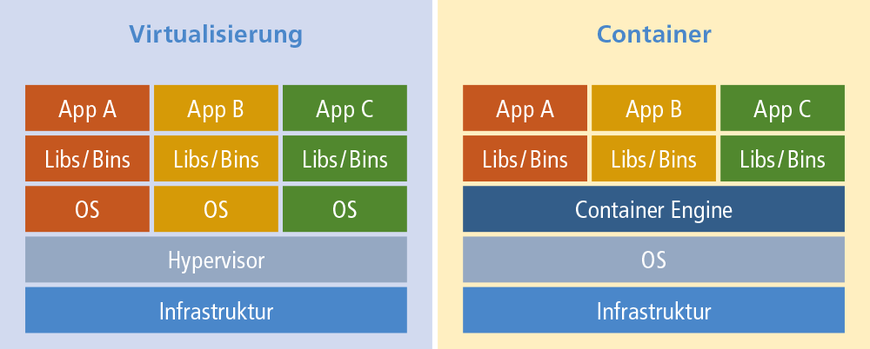
\includegraphics[width=0.8\textwidth]{pics/Container_VM.png}
  \centering
  \caption{Unterschied von Virtuellen Maschinen und Containern von https://www.shd-online.de/fachartikel/der-app-store-fuer-server-wofuer-sie-container-brauchen/}
\end{figure}

\subsection{Dockerfile}
Jeder Docker-Container beginnt mit einem Dockerfile. Diese Textdatei enthält eine 
Reihe von Anweisungen zur Erstellung eines Docker-Abbilds, einschließlich des Betriebssystems, 
der Sprachen, der Umgebungsvariablen, der Dateispeicherorte, der Netzwerk-Ports und aller anderen 
Komponenten, die zur Ausführung benötigt werden.

\begin{figure}[H]
  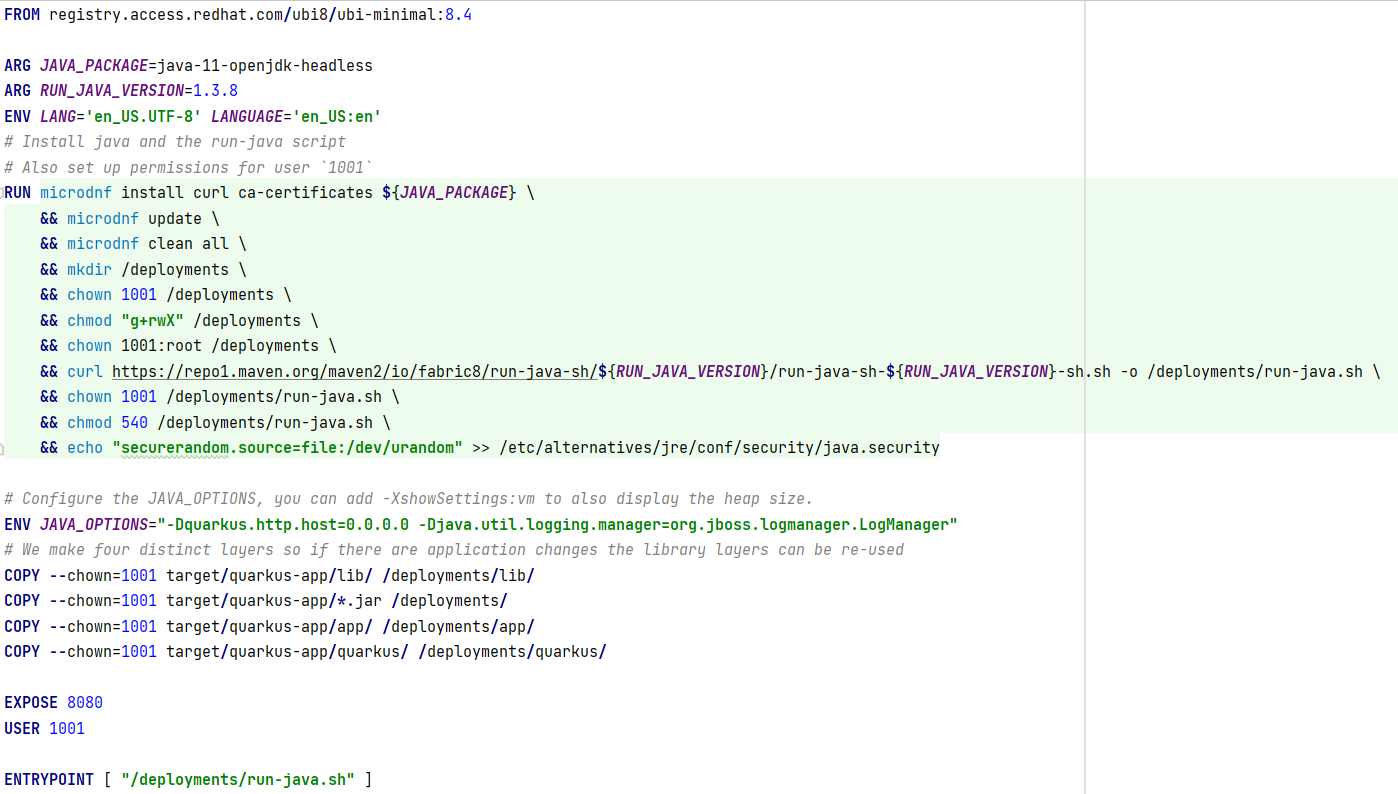
\includegraphics[width=0.8\textwidth]{pics/Bsp_Dockerfile.PNG}
  \centering
  \caption{Beispiel eines Dockerfiles}
\end{figure}

\subsection{Container-Images}
Ein Docker-Image ist eine andere Möglichkeit einen Docker-Container zu erstellen.
Ein Docker-Image ist eine portable, schreibgeschützte, ausführbare Datei, die die Anweisungen zur 
Erstellung eines Containers und die Spezifikationen dafür enthält, welche Softwarekomponenten der 
Container wie ausführen wird. Jeder Container ist eine Instanz eines Images, wobei mehrere Instanzen 
desselben Images gleichzeitig ausgeführt werden können. Diese Cluster von Containern müssen dann orchestriert werden, 
wozu in der Regel Kubernetes eingesetzt wird. \cite{noauthor_docker_nodate-2}

\subsubsection{Kubernetes}
Kubernetes ist eine flexible, erweiterbare Open-Source-Plattform für die Verwaltung von
containerisierten Systemen und Diensten, die sowohl eine deklarative Konfiguration als auch eine 
Automatisierung ermöglicht. \cite{noauthor_kubernetes_2021}, \cite{noauthor_was_nodate-7}

\begin{itemize}
  \item Automatisierte Terminplanung
  \item Automatisierte Rollouts und Rollbacks
  \item Horizontale Skalierung und Lastausgleich
  \item Bietet eine konsistente Umgebung für Entwicklung, Tests und Produktion
  \item Automatisch skalierbare Infrastruktur
\end{itemize}

\subsection{Docker run}
Docker run ist der Befehl von Docker, mit dem ein Container gestartet wird.
Es können Spezifikationen zum Beispiel für den Namen des Containers und den Port, auf dem der Container
laufen soll, getroffen werden.

\subsection{Docker Hub}
Docker Hub ist ein Repository, in dem Container-Images gespeichert, freigegeben und verwaltet werden 
können. Es ist mit den GitHub-Repository für GitHub zu vergleichen, nur werden im Docker Hub Images 
zur Verfügung gestellt. Startet man einen Container eines Images wird mit den Standardeinstellungen dieses 
Image automatisch auf Docker Hub gesucht und wenn gefunden, heruntergeladen. \cite{noauthor_docker_nodate-1}

\subsection{Docker-Engine}
Die Docker-Engine ist die zugrunde liegende Client-Server-Technologie, die 
Container erstellt und ausführt. Die Docker-Engine umfasst einen 
langlaufenden Daemon-Prozess zur Verwaltung von Containern, APIs, die es 
Programmen ermöglicht, mit dem Docker-Daemon zu kommunizieren, sowie eine 
Befehlszeilenschnittstelle bildet.

\subsection{Docker Compose}
Docker Compose ist ein Tool, das YAML-Dateien verwendet, um Multicontainer-Docker-Anwendungen 
zu definieren und auszuführen. Es ermöglicht Ihnen, alle Dienste Ihrer Konfiguration zu erstellen, 
zu starten, zu stoppen und neu zu erstellen und den Status und die Protokollausgabe 
aller laufenden Dienste anzuzeigen.

\subsubsection{YAML}
YAML ist eine für Sprache zur Daten-Serialisierung. Sie wird üblicherweise für Konfigurationsdateien 
und in Anwendungen verwendet, in denen Daten gespeichert oder übertragen werden. YAML verwendet Schlüssel-Wert-Paaren. \cite{noauthor_yaml_2022}, \cite{noauthor_einfuhrung_2021}

\begin{figure}[H]
  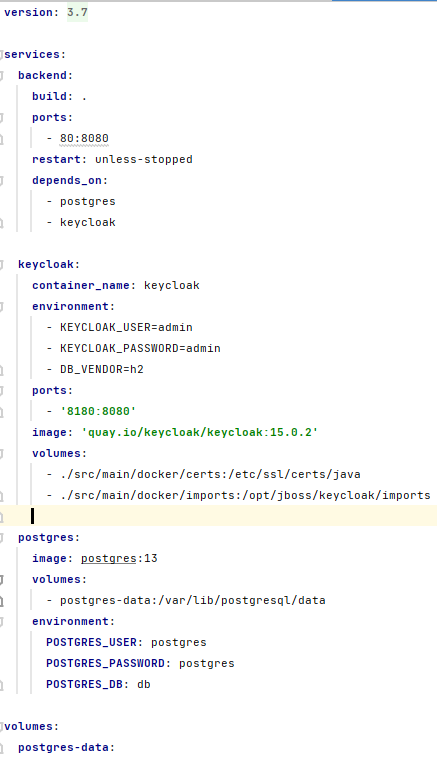
\includegraphics[width=0.6\textwidth]{pics/Bsp_Docker-composeYML.PNG}
  \centering
  \caption{Beispiel für Docker Compose YAML-Datei}
\end{figure}

\subsection{Docker Desktop}
Docker Desktop vereint all diese Komponenten in einer Anwendung, die eine 
benutzerfreundliche Möglichkeit zur Erstellung und gemeinsamen Nutzung von containerisierten 
Anwendungen und Microservices bietet. \cite{noauthor_docker_nodate-3}, \cite{noauthor_install_nodate-1}

\section{Keycloak}
\begin{wrapfigure}{r}{0.3\textwidth}
  \begin{center}
    
\includegraphics[width=0.2\textwidth]{pics/KeyCloak_logopng.png}
    \caption{Keycloak Logo von https://www.gepardec.com/keycloak/}
  \end{center}
\end{wrapfigure}
Keycloak ist ein Open-Source-Identitäts- und Zugriffsmanagement-Tool mit dem Schwerpunkt auf 
modernen Anwendungen wie Single-Page-Anwendungen, mobilen Anwendungen und REST-APIs.
Mit der Verwendung von Keycloak authentifizieren sich Benutzer mittels des Keycloak und nicht mit 
individuellen Anwendungen. Das bedeutet, dass keine Login-Formulare, Authentifizierung von Benutzern 
und Speicherung von Benutzern implementiertet werden müssen. Diese Login-Seite kann sogar angepasst werden.
Nach einmaligen Einloggen bei Keycloak, müssen sich die Benutzer nicht erneut anmelden, um auf 
eine andere Anwendung zuzugreifen. Dasselbe gilt auch für die Abmeldung. Mit der Verwendung von
Single-Sign-Out müssen sich Benutzer nur einmal abmelden um von allen Anwendungen, 
die den Keycloak benutzen, abgemeldet zu werden.  
\newline
\newline
Eine zusätzliche Funktion des Keycloak ist die eingebaute Unterstützung, um sich mittels LDAP mit 
bestehenden Active-Directory-Servern zu verbinden. 
Docker stellt ein Image für Keycloak zur Verfügung. \cite{noauthor_keycloak_nodate-1}, \cite{noauthor_quarkus_nodate}, \cite{noauthor_keycloakkeycloak_nodate}, \cite{noauthor_keycloak_2022}, \cite{noauthor_mit_2020}

\subsection{LDAP}
LDAP oder ausgeschrieben Lightweight Directory Access Protocol ist ein Softwareprotokoll, 
das Daten speichert und sortiert, um sie leicht auffindbar zu machen. Bei den Daten kann es 
sich um beliebige Informationen über Geräte oder Benutzer handeln, die in Verzeichnissen 
gespeichert sind. LDAP ist das Protokoll, das von Servern verwendet wird, um mit den 
Verzeichnissen vor Ort zu kommunizieren.
\newline
\newline
Der Hauptnutzen von LDAP besteht darin, als zentraler Mittelpunkt für die Authentifizierung und 
Autorisierung zu dienen. LDAP hilft dabei Benutzernamen und Kennwörter zu speichern und später 
wieder abrufbar zu machen, zum Beispiel wenn ein Benutzer versucht, auf eine LDAP-fähige Anwendung 
zuzugreifen. Mithilfe der in LDAP gespeicherten Anmeldeinformationen 
wird der Benutzer authentifiziert.
\newline
\newline
In LDAP können auch Benutzerattribute gespeichert werden, die bestimmen, worauf der Benutzer 
zugreifen darf. Obwohl LDAP und Active-Directory (AD) häufig synonym verwendet werden, 
handelt es sich um zwei verschiedene Arten von Software, die jedoch zusammenarbeiten können. \cite{bar_was_nodate}, \cite{noauthor_lightweight_nodate}, 

\subsection{Active-Directory}
Active-Directory (AD) ist eine Datenbank und bietet eine Reihe von Diensten, die Benutzer mit den 
Netzwerkressourcen verbinden. Die Datenbank beziehungsweise das Directory enthält wichtige Informationen 
über Ihre Umgebung, zum Beispiel welche Benutzer und Computer es gibt und wer was tun darf. \cite{noauthor_active_nodate}, \cite{noauthor_lightweight_2022}, \cite{noauthor_active_nodate-1}, \cite{noauthor_was_nodate-8}

Active-Directories bestehen aus drei Hauptebenen: 
\begin{enumerate}
  \item Domänen
  \item Bäume
  \item Wälder
\end{enumerate}

Eine Domäne ist eine Gruppe zusammengehöriger Benutzer, Computer und anderer Objekte. 
Mehrere Domänen können zu einem Baum (tree) zusammengefasst werden, und mehrere Bäume können zu 
einer Gesamtstruktur (auch Forest genannt) gruppiert werden.

\subsection{Login Prozess}
\begin{figure}[H]
  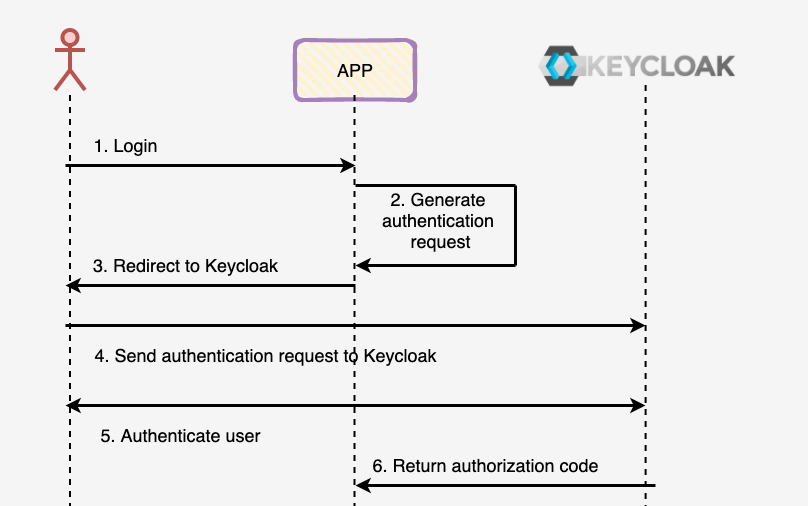
\includegraphics[width=0.8\textwidth]{pics/Keycloak_Auth.png}
  \centering
  \caption{Login Prozess von https://medium.com/codex/introduction-to-keycloak-227c3902754a}
  \label{fig:keycloak1}
\end{figure}

In der Abbildung (siehe Abb. \ref{fig:keycloak1}) wird der Login-Prozess des KeyCloak vereinfachend dargestellt.
\begin{enumerate}
  \item Der Benutzer klickt auf einen Login-Button
  \item Die Anwendung generiert eine Authentifizierungsanfrage.
  \item Die Authentifizierungsanforderung wird an den Benutzer gesendet.
  \item Der Keycloak zeigt dem Benutzer die Anmeldeseite an. Der Benutzer gibt seinen Benutzernamen und sein Passwort ein und schickt das Formular ab
  \item Keycloak überprüft die Anmeldedaten und erstellt daraufhin einen Autorisierungscode, der an die Anwendung zurückgeschickt wird
  \item Autorisierungscode wird gegen das ID-Token und das Refresh-Token ausgetauscht
\end{enumerate}

\subsubsection{JSON-Web-Token (JWT)}
Der Keycloak sendet standardmäßig ein signiertes JSON-Web-Token (JWT).
JSON Web Token (JWT) ist ein offener Standard, der eine kompakte Methode zur sicheren 
Übertragung von Informationen zwischen Parteien in Form eines JSON-Objekts ermöglicht. 
Es wird hauptsächlich für Authentifizierung und Informationsaustausch verwendet.
Diese Informationen können überprüft werden und sind vertrauenswürdig, da sie digital signiert werden.
JWTs können aber auch verschlüsselt werden, um die Geheimhaltung zwischen den Parteien zu gewährleisten. \cite{auth0com_jwtio_nodate}, \cite{noauthor_json_nodate}, \cite{noauthor_json_nodate-1}
 
\subsection{Admin Console}
Über die Admin Konsole können alle Aspekte des Keycloak-Servers zentral verwaltet werden.
Die verschiedene Einstellungen können hier getroffen und Funktionen aktiviert und deaktiviert werden. 
Weiters können Identitäts-Brokering und Benutzer-Föderation konfiguriert werden. Zudem besteht die Möglichkeit 
Anwendungen und Dienste zu erstellen und zu verwalten und feinkörnige Autorisierungsrichtlinien zu definieren.
Einstellungen von Benutzer, einschließlich Berechtigungen und Sitzungen können ebenfalls getroffen werden. \cite{noauthor_keycloak_nodate}, \cite{noauthor_server_nodate}

\begin{figure}[H]
  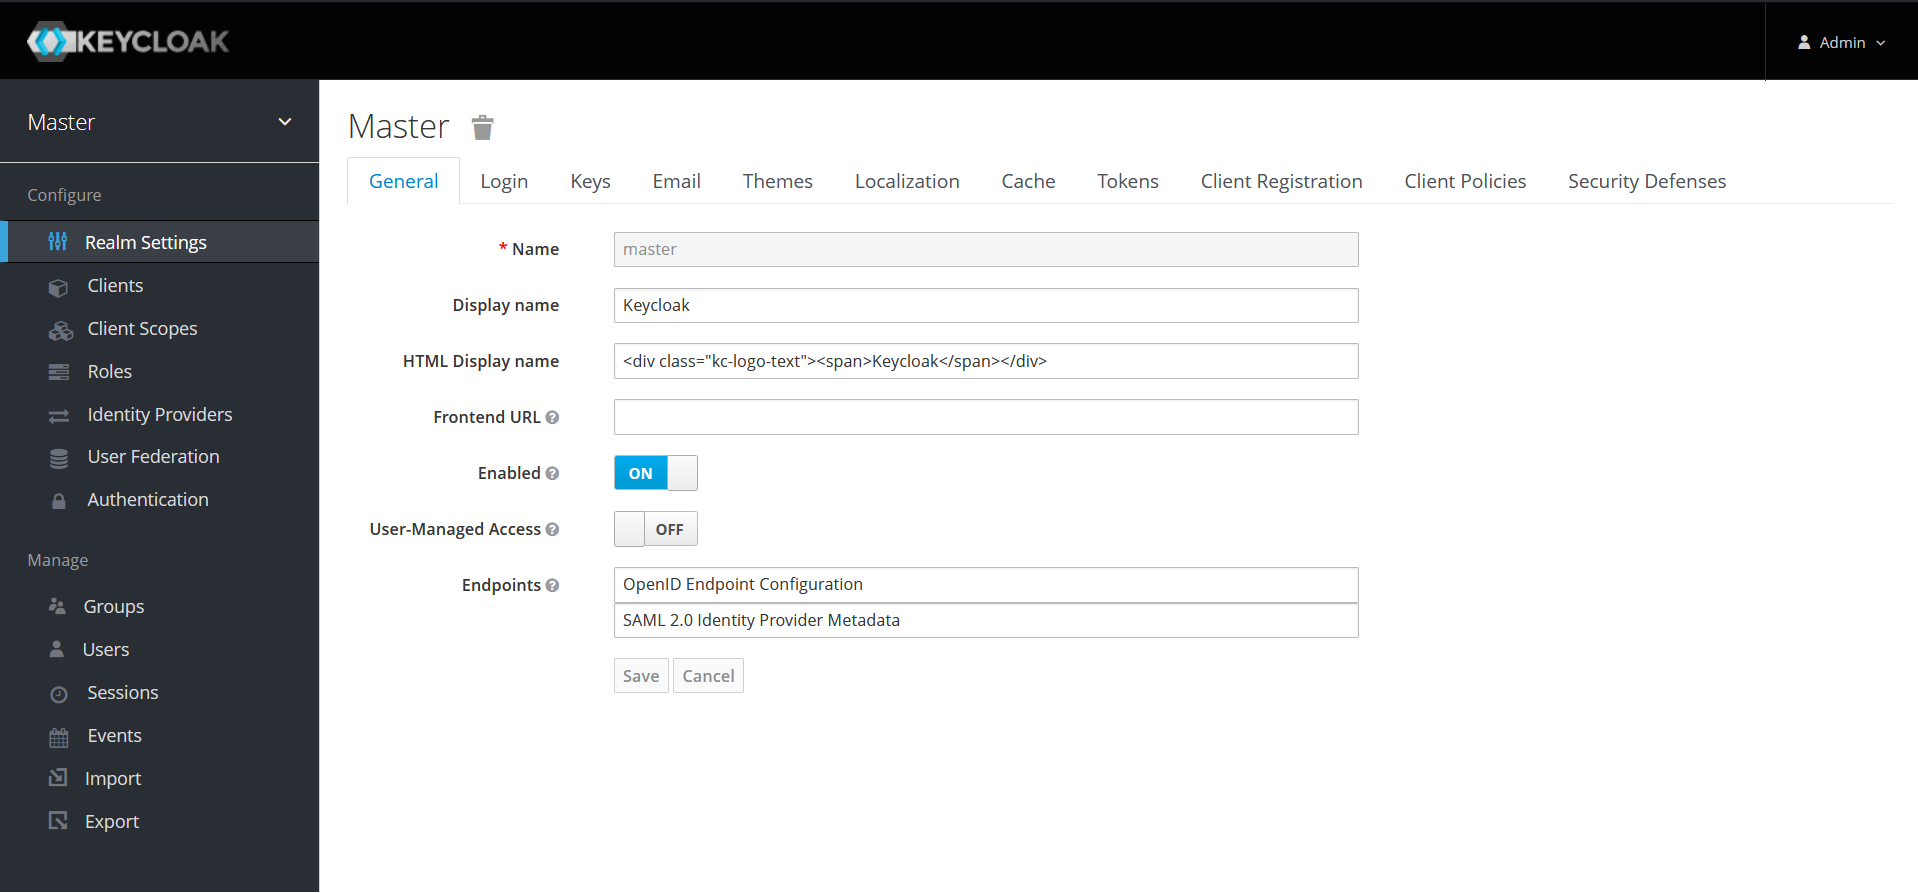
\includegraphics[width=1.0\textwidth]{pics/Keycloak_AdminConsole.PNG}
  \centering
  \caption{Admin Console}
\end{figure}

\subsection{Keycloak Konto-Konsole}
Die Konsole ist für Benutzer. Dort können sie ihr Konto verwalten, z.B. ihr Profil und ihr 
Passwort aktualisieren.

\section{Traefik}
\label{cha:treafik}
\setauthor{Raffeiner Christine}
Traefik ist ein Open Source Edge Router, der die Veröffentlichung von Diensten vereinfacht. 
Der Router empfängt Anfragen stellvertretend für das System und findet heraus, welche Komponenten für deren Bearbeitung 
zuständig sind. Traefik ist kompatibel mit allen wichtigen Cluster-Technologien wie Kubernetes, Docker, Docker Swarm, AWS, 
Mesos und Marathon. 
\newline
\newline
Was Traefik neben seinen vielen Funktionen auszeichnet, ist, dass es automatisch Dienste im Netzwerk erkennt, auch wenn diese nachträglich gestartet werden. 
Traefik inspiziert die Infrastruktur des Systems und findet heraus, welcher Dienst für welche 
Anfragen zuständig ist und kann diese in Echtzeit abfangen und anpassen (z.B. https auf http). 
Traefik benötigt keine separate Konfigurationsdatei um das System zu verwalten und zu synchronisieren: 
Alles geschieht automatisch und in Echtzeit ohne Neustarts und Verbindungsunterbrechungen. \cite{noauthor_traefik_nodate}, \cite{noauthor_traefiktraefik_nodate}
\begin{figure}[H]
  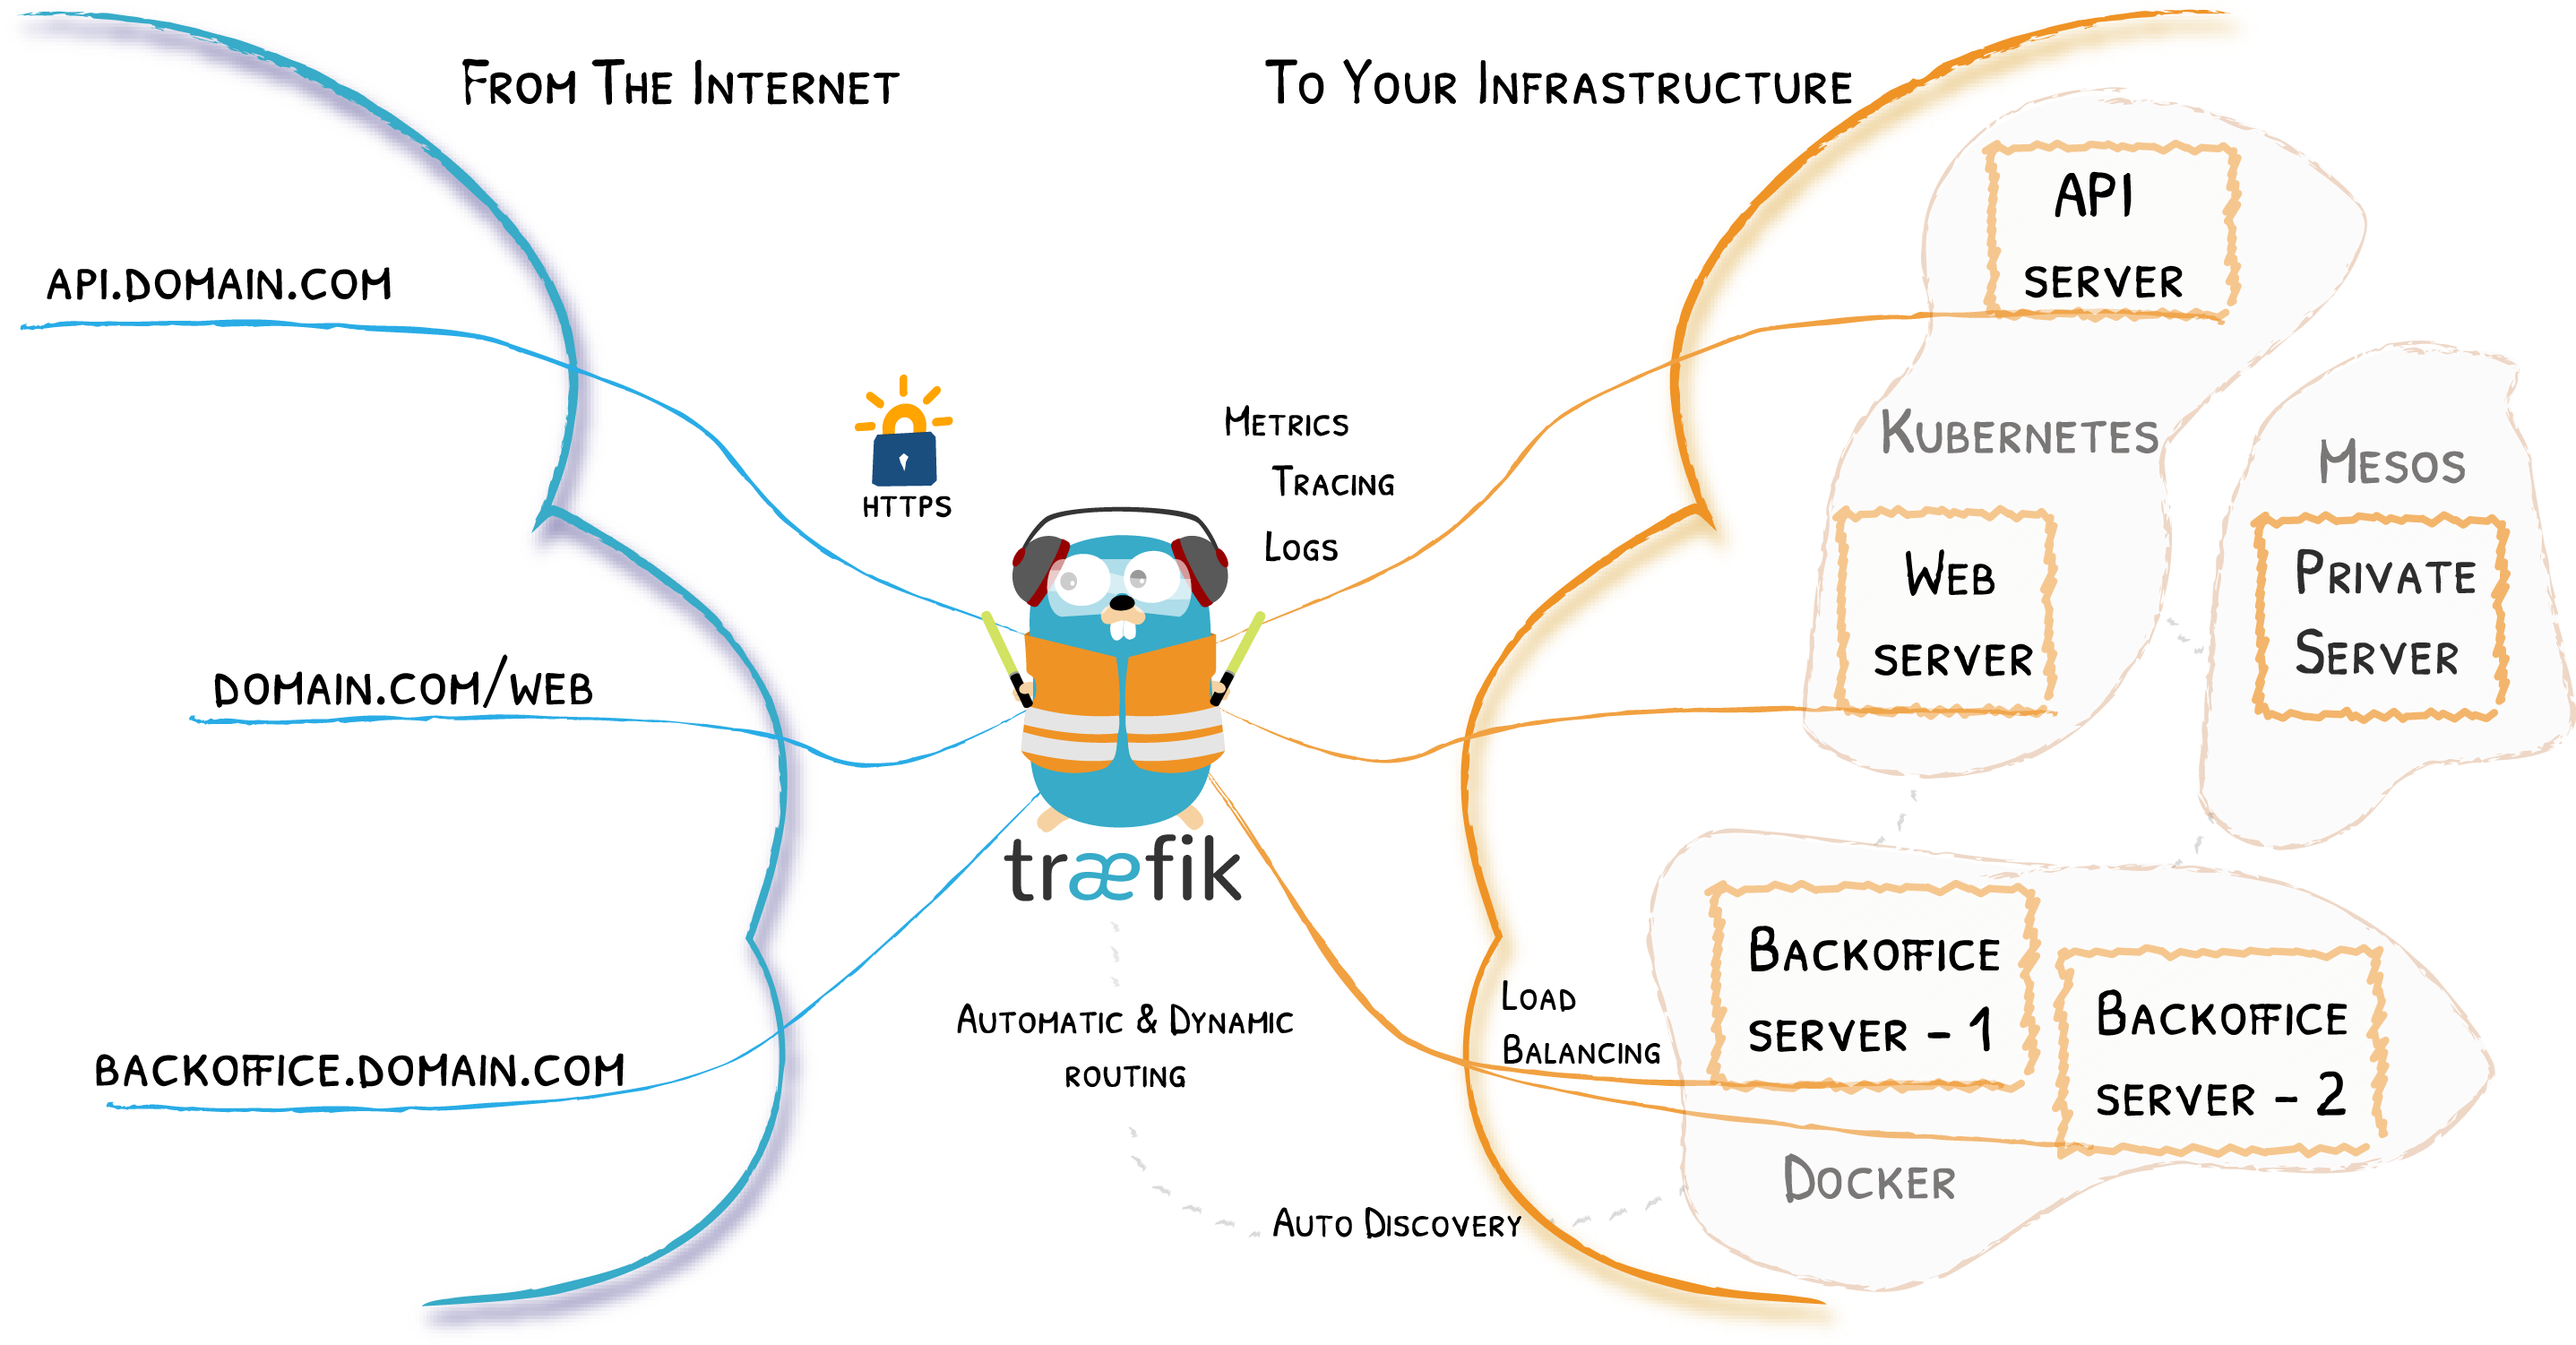
\includegraphics[width=0.9\textwidth]{pics/traefik-architecture.png}
  \centering
  \caption{Funktionsweise Traefik}
\end{figure}

\section{PlantUML}
\label{chap:plantuml}

\begin{figure}[!htb]
        
\includegraphics[width=0.2\textwidth]{pics/PlantumlLogo.png}
        \centering
        \caption{PlantUML Logo source: \cite{noauthor_plantuml_nodate}}
\end{figure}
PlantUML ist ein Open-Source-Werkzeug, mit dem Benutzer/innen Diagramme aus einer einfachen Textsprache 
erstellen können. Neben verschiedenen UML-Diagrammen unterstützt PlantUML auch verschiedene andere 
Formate für die Softwareentwicklung. \cite{noauthor_plantuml_2022}

\subsection{PlantUML integration}
Das Plugin PlantUML integration wird von IntelliJ verwendet um die PlantUML-Dateien anzuzeigen und zu erstellen.
Das Plugin bietet Code-Navigation und Hervorhebung. \cite{noauthor_plantuml_nodate}

\section{Markdown}
\label{chap:markdown}
\begin{figure}[!htb]
        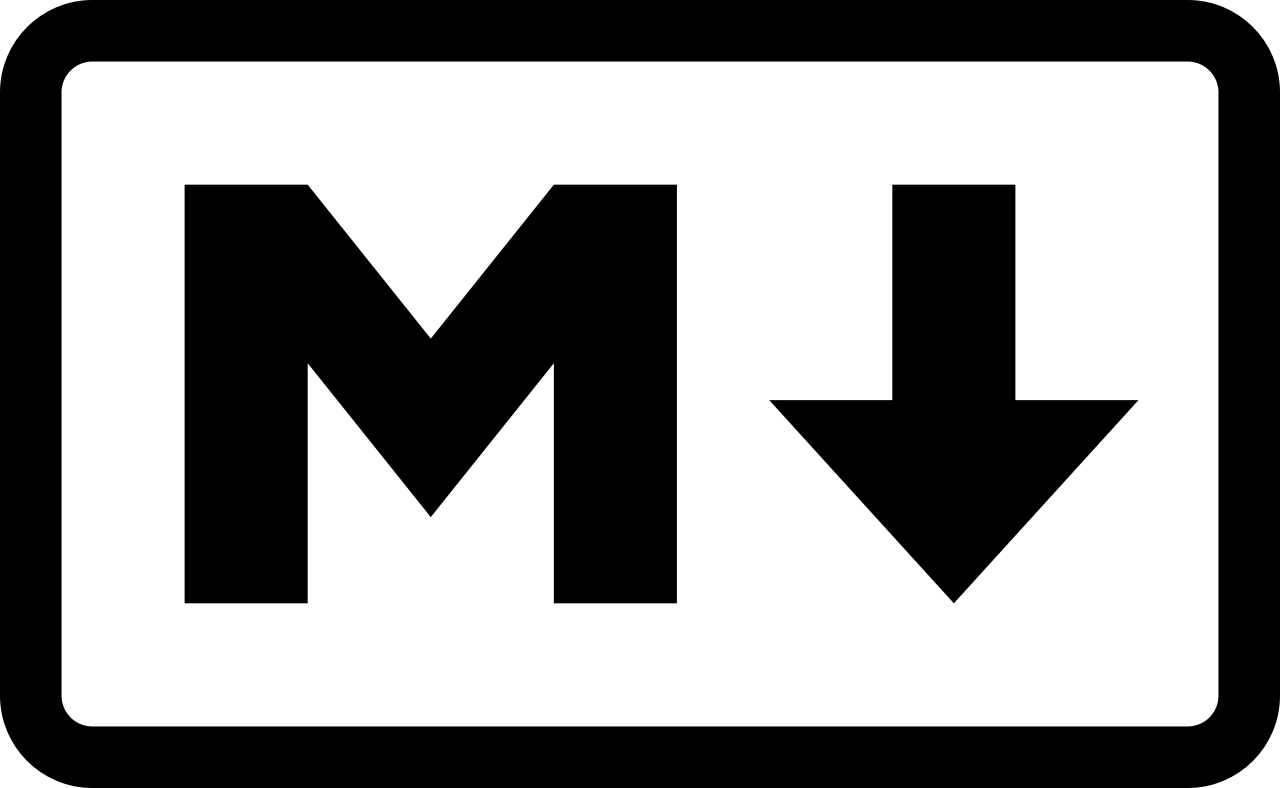
\includegraphics[width=0.2\textwidth]{pics/MarkdownLogo.png}
        \centering
        \caption{Markdown Logo 
        source: \cite{noauthor_markdown_2021} }
\end{figure}

Markdown ist eine leichtgewichtige Auszeichnungssprache, mit der 
Formatierungselemente zu Textdokumenten im Klartext hinzufügen werden können. \cite{noauthor_markdown_2021}, \cite{noauthor_markdown_nodate}

\section{Java}
\setauthor{Weissengruber Nina}
\begin{wrapfigure}{r}{0.3\textwidth}
    \begin{center}
      
\includegraphics[width=0.2\textwidth]{pics/Java_Logo.png}
      \caption{Java Logo ~\cite{java_logo}}
    \end{center}
\end{wrapfigure}
Java ist eine objektorientierte Programmiersprache, die in vielen Teilen der Informatik verwendet wird. 
Java als Programmiersprache dient vor allem zum Formulieren von Programmen. Anfangs liegen die Programme in 
Quellcode, also in für Menschen verständlichen Text vor. Mithilfe des Java-Compilers wird der Quellcode in für
Maschinen verständlichen Bytecode übersetzt. Dieser Quellcode wird dann über die Java Virtual Machine (JVM)
ausgeführt. ~\cite{java}
\newline
\newline
Ein großer Vorteil von Java ist die Plattformunabhängigkeit. Zum Ausführen der Programme oder Anwendungen
wird kein bestimmtes Betriebssystem benötig sondern lediglich die Java-Laufzeitumgebung (JRE).
Diese Laufzeitumgebung ist bereits auf vielen Computern mit verschiedenen Betriebssystemen vorinstalliert, 
wodurch die Plattformunabhängigkeit gegeben ist. Die Plattformunabhängigkeit wird auch durch die Java
Virtuell Machine (JVM) realisiert. ~\cite{java_biteno}
\subsection{Java Runtime Environment}
Die Java Runtime Environment (JRE) oder auch Java Laufzeitumgebung oder Java Runtime ist Teil des Java 
Development Kits (JDK).
\newline
\newline
Eine Laufzeitumgebung verhält sich wie ein kleines Betriebssystem und stellt alle notwendigen
Funktionalitäten für die Ausführung eines Programmes bereit. Die Laufzeitumgebung lädt Anwendungen und
lässt diese auf einer Plattform laufen, auf der alle notwendigen Ressourcen für einen 
betriebsystemunabhängigen Betrieb zu Verfügung.
\newline
\newline
Eine laufende Anwendung interagiert über ein Runtime System mit der Laufzeitumgebung. 
Die Laufzeitumgebung wiederum dient als Vermittler zwischen Anwendung und Betriebssystem. 
Die JRE stellt verschiedene Funktionen für Speicher, Netzwerk und Hardware bereit.
Diese Funktionen werden von der Laufzeitumgebung ausgeführt und nicht von der Anwendung und arbeiten 
unabhängig vom Betriebssystem. 
\newline
\newline
Ein großer Vorteil der Laufzeitumgebung ist, dass Programme Zugriff auf alle benötigten Funktionen haben, 
jedoch unabhängig von Betriebssystem arbeiten.
~\cite{java_jre}

\subsection{Java Development Kit}
Das Java Development Kit (JDK) bildet die Grundlage, auf der Anwendungen aufgebaut werden. 
JDK besteht aus verschiedenen Softwarekomponenten und enthält eine Vielzahl von Tools und Dienstprogrammen, 
mit denen verschiedene Aufgaben ausgeführt werden können. 
Die Hauptverwendung von JDK besteht darin, Code von Java-Code in Bytecode zu kompilieren,
wobei die JRE verwendet wird, um den Bytecode auszuführen.
~\cite{java_jdk}

\subsection{Java Virtual Machine}
Die Java Virtual Machine (JVM) ist die zentrale Komponente der Java-Laufzeitumgebung (JRE). 
Die JVM ermöglicht die plattformunabhängige Ausführung von Programmen im Java-Bytecode. 
Die JVM ist eine prozessbasierte VM oder auch ein einfacher virtueller Computer, in dem Java-Bytecode
ausgeführt wird. Die VM übersetzt die Anweisungen des Bytecodes zur Laufzeit in Maschinencode.
\newline
\newline
Ein weiterer Vorteil der JVM ist die Geschwindigkeit und Sicherheit. Da die Java-Programme von den 
Betriebssystemen abgeschottet sind, wird die Sicherheit erhöht, da Zugriffe auf Ressourcen sich genau
kontrollieren lassen.
~\cite{java_jvm}

\section{Quarkus}
\setauthor{Weissengruber Nina}
\begin{wrapfigure}{r}{0.3\textwidth}
    \begin{center}
      
\includegraphics[width=0.4\textwidth]{pics/Quarkus_logo.jpg}
      \caption{Quarkus Logo ~\cite{quarkus_logo}}
    \end{center}
\end{wrapfigure}

Quarkus ist ein Java Framework für JVMs (Java Virtual Machines) und native Kompilierung, um Java-Anwendungen 
für Container und Clouds zu optimieren.
~\cite{quarkus_redhat}

Quarkus unterstützt 2 Modi:
\begin{enumerate}
\item Optimierung des Bytecodes und Ausführen in der JVM

Java Code, der mit Quarkus geschrieben wurde, kann auf der JVM ausgeführt werden.
Es gibt jedoch Vorteile in Hinsicht auf den Speicherverbrauch und die Startzeit der laufenden Anwendung.
Um dies zu ermöglichen, schiebt Quarkus eine Reihe von zeitaufwendigen Schritten in den Build-Prozess.
Unteranderem:

   \begin{itemize}
     \item Laden und Parsen von Konfigurationen
     \item  Scannen des Java-Klassen-Pfades und das Auflösen von Annotationen
     \item  gegebenenfalls das Erstellen von Entitäten-Modellen für Datenanken
   \end{itemize}

   Quarkus führt diese Schritte einmalig durch und speichert die Ergebnisse für einen schnellen Abruf zwischen.
   \newline
   Unter anderem reduziert Quarkus die Menge der zur Laufzeit dynamisch vorliegenden Informationen. 
   Diese Informationen werden durch entsprechende Konstrukte ersetzt, 
   was im Hinblick auf den Einsatz mit Containern sinnvoll ist. 

\item Ausführen als nativer Code nach Kompilierung

Mit der Ahead-of-time-compilation (AOT) wird aus dem Java-Quelltext kein Bytecode erzeugt, 
sondern direkt ausführbarer Maschinencode. Dies bedeutet, dass auf der Ziel-Hardware keine JVM benötigt wird.
\end{enumerate}
~\cite{quarkus_ionos}

\subsubsection{Ahead-of-time compilation}
Bei der Ahead-of-time (AOT) compilation wird der Programmcode bereits zur Compilezeit/Kompilierzeit in Maschinensprache
übersetzt.
\newline
Mithilfe der AOT compilation wird die Startzeit der JVM von Java-Programmen verbessert.
~\cite{ahead_of_time_compilation}

\section{PostgreSQL}
\setauthor{Weissengruber Nina}
\begin{wrapfigure}{r}{0.3\textwidth}
    \begin{center}
      
\includegraphics[width=0.4\textwidth]{pics/postgreSql_Logo.png}
      \caption{PostgreSql Logo ~\cite{postgre_sql_logo}}
    \end{center}
\end{wrapfigure}
PostgreSQL ist ein leistungsstarkes, objektrelationales Open-Source-Datenbanksystem.
PostgreSQL basiert auf dem Client-Server-Modell, dies bedeutet,
dass ein am Server laufender Prozess die Datenbankdateien und deren Verbindungen, 
die von Client zum Server aufgebaut werden, und bearbeitete Anfragen verwaltet.
~\cite{postgre_sql}
\newline
\newline
Ein Vorteil von PostgreSQL ist, dass es ein Open Source System ist. Somit ist der Code frei zugänglich,
daher ist es möglich, PostgreSQL zu nutzen oder so zu verändern und implementieren,
wie es aktuell für einen von Vorteil ist. Weites ist es möglich, die PostgreSQL Datenbank zu skalieren und
somit kann die Datenbank auf die Größe der Anwendung angepasst werden.
~\cite{postgre_sql_cybertec}

\section{Rest-API}
\setauthor{Weissengruber Nina}
Representational State Transfer - Application Programming Interface (Rest-API) ermöglicht den Austausch von
Informationen, die sich auf unterschiedlichen Systemen befinden. Eine Rest-API ist zustandslos, dies bedeutet,
dass Aufrufe unabhängig voneinander erfolgen und jeder Aufruf alle Daten enthält, 
die erforderlich sind für eine erfolgreiche Durchführung.
~\cite{rest_api_ryte}
\newline
\newline
Außerdem baut Rest-API auf bestehende Systeme und Funktionen des Hypertext Transfer Protocol (HTTP) auf. 
Somit können Rest-basierte Interaktionen deren Status über numerische HTTP-Statuscodes kommunizieren. 
Der Vorteil besteht darin, dass REST-APIs diese HTTP-Statuscodes verwenden, um Fehler zu erkennen.
\newline
\newline
Weiters ist Rest-API Sprachunabhängig, dies bedeutet, dass man beim Erstellen von Restful-APIs oder 
Webdiensten jegliche Sprache verwenden kann, die HTTP verwendet. 
~\cite{rest_api_tech_target}
\newline
\newline
\begin{figure}[!htb]
  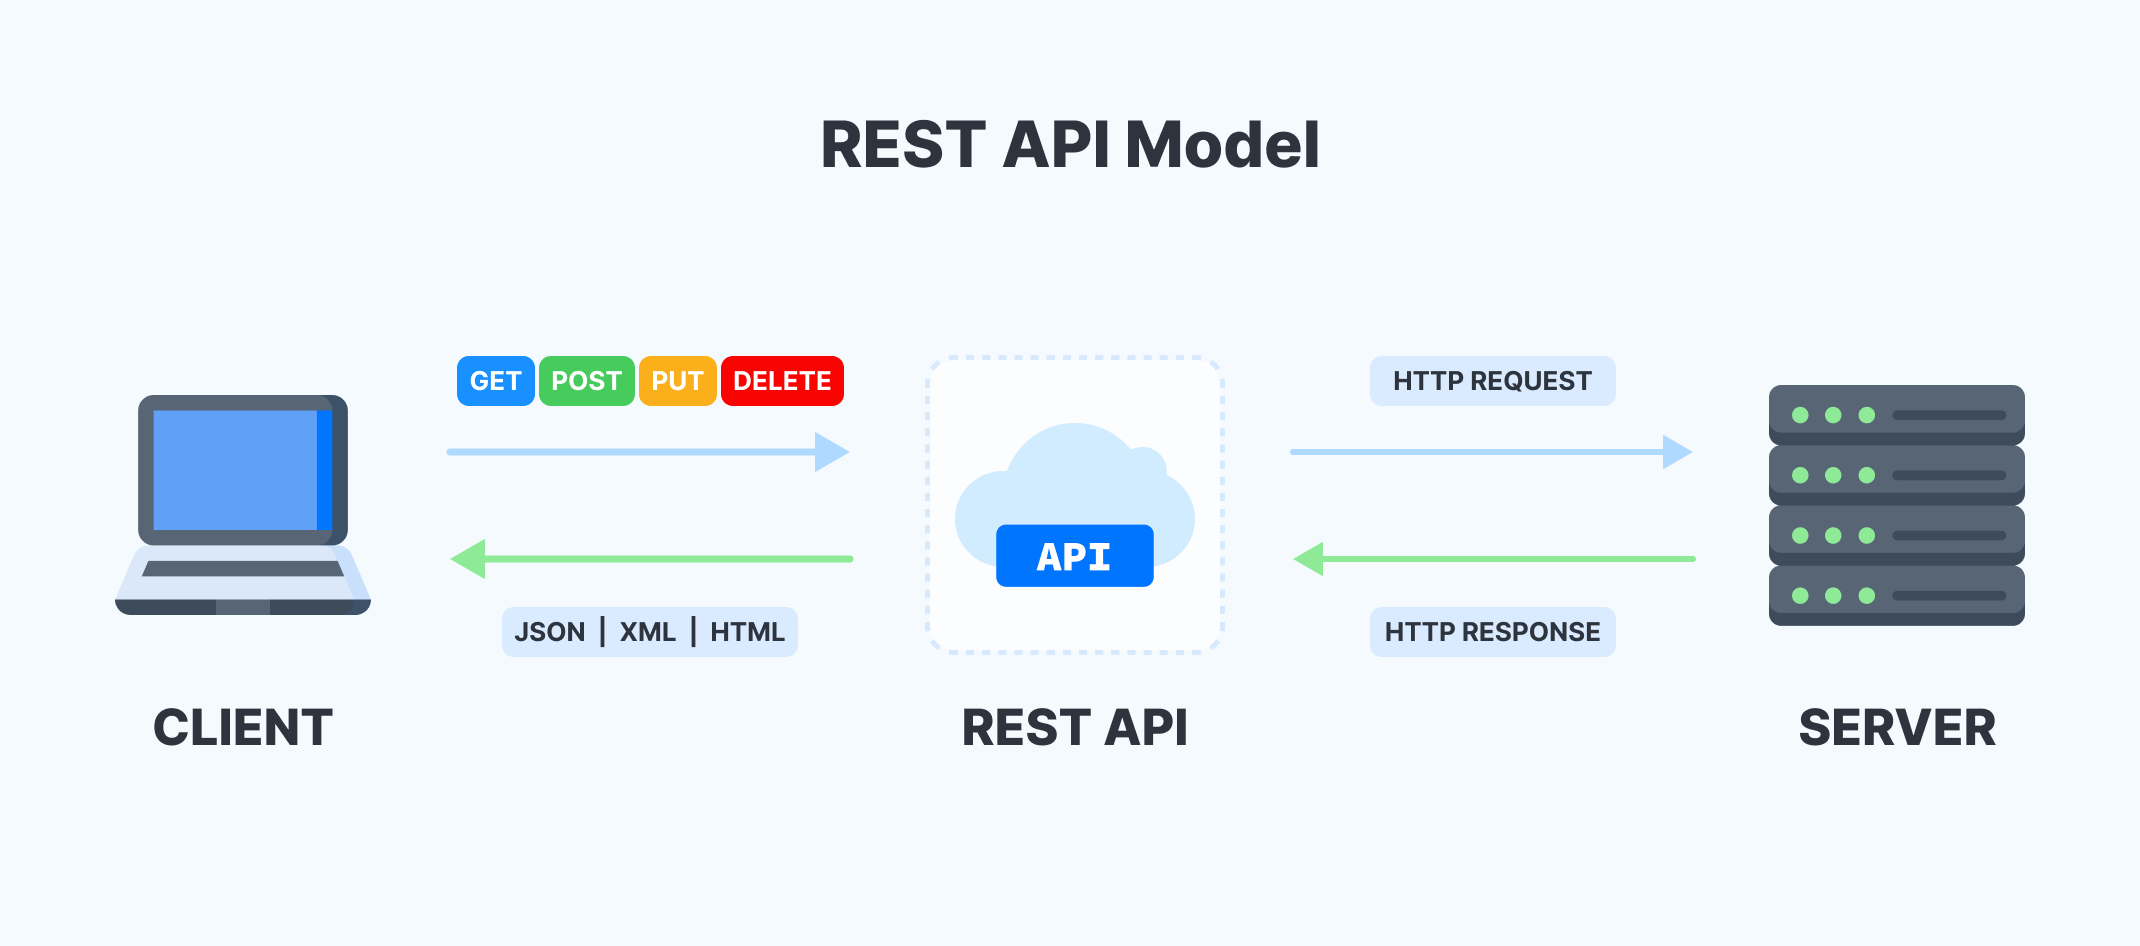
\includegraphics[width=0.8\textwidth]{pics/api-rest-model.png}
  \centering
  \caption{Rest-API Model ~\cite{rest_api_model}}
\end{figure}
\newline
Der Client schickt mittels HTTP-Request Methoden Anfragen an die Rest-API, die die Requests an den Client
weiterschicken.
\newline
Der Server sendet einen HTTP-Response an die Rest-API welche die Response an den Client als JSON,
XML oder HTML Datei sendet.

\subsection{API}
Ein Application Programming Interface (API) ist eine Schnittstelle, die verschiedene Programme verbindet
und die Datenübertragung und den Austausch von Anweisungen zwischen Programmteilen standardisiert.
\newline
APIs bieten verschiedene Anwendungsbereiche, über welche unterschiedliche Aufgaben ausgeführt werden können.
\newline
Es gibt vier verschiedene Arten von APIs:
\begin{itemize}
  \item Funktionsorientierte APIs
  \item Dateiorientierte APIs
  \item Protokollorientierte APIs
  \item Objektorientierte APIs
\end{itemize}

Funktionsorientierte APIs sind komplexe Schnittstellen, die es ermöglichen, auf Hardware-Komponenten
zuzugreifen. Dateiorientierte APIs ermöglichen die Verbindung auf Dateiebene und damit können Daten
abgefragt und geschrieben werden. Protokollorientierte APIs werden zur standardisierten Kommunikation 
zwischen Programmen verwendet. Objektorientierte APIs sind flexibel und können in verschiedenen Bereichen 
eingesetzt werden.
~\cite{api}

\subsection{HTTP}
Hypertext Transfer Protocol (HTTP) ist ein Protokoll, mit dem Daten in Netzwerken übertragen werden. 
HTTP ist standardisiert und definiert, wie Webclient und Server miteinander kommunizieren, 
damit vom Client angeforderte Daten geladen und angezeigt werden.
\newline
\newline
HTTP definiert zwei unterschiedliche Arten von Nachrichten

\begin{itemize}
  \item Anfrage (Request)
  \item Antwort (Response)
\end{itemize}

Diese Nachrichten bestehen aus einem HTTP-Header und einem HTTP-Body. 
Im Header sind Meatinformationen enthalten und im Body befinden sich die Daten, 
die an den Client geschickt werden.
\newline
\newline
Zur Übertragung von Daten zwischen Server und Client wird das TCP/IP-Protokoll verwendet. 
Fordert der Client über TCP ein Dokument an, wird eine Antwort (Response) vom Server versendet,
dabei wird auch ein HTTP-Statuscode mitgesendet. Mithilfe des Statuscodes wird Auskunft darüber gegeben,
ob die Anfrage erfolgreich war. Je nachdem, ob es erfolgreich war oder nicht wird ein dreistelliger
HTTP-Code an den Client gesendet.
~\cite{http_ryte}

\subsubsection{HTTP-Statuscodes}
HTTP-Statuscodes zeigen an, ob eine HTTP-Anfrage (Request) erfolgreich abgeschlossen wurde.

Man unterscheidet zwischen folgenden Statuscodes:
\begin{itemize}
  \item Informative Antworten (100-199)
  \item Erfolgreiche Antworten (200-299)
  \item Umleitungen (300-399)
  \item Client-Fehler (400-499)
  \item Server-Fehler (550-599)
\end{itemize}
~\cite{http_statuscode}

\begin{figure}[!htb]
  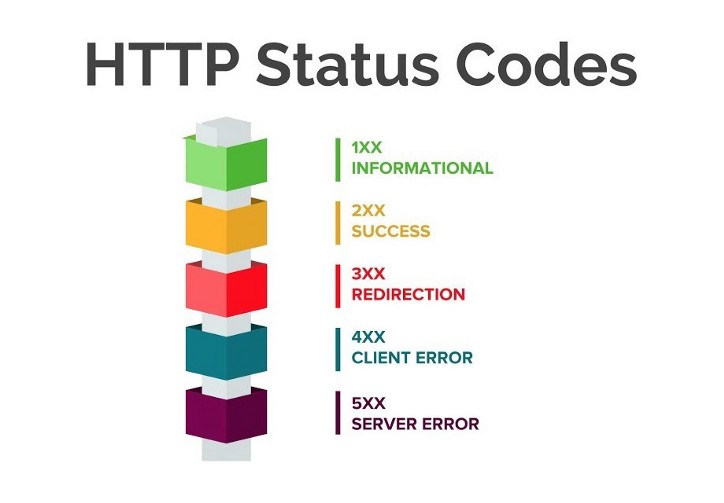
\includegraphics[width=0.8\textwidth]{pics/httpStatusCodes.jpeg}
  \centering
  \caption{HTTP-Statuscodes ~\cite{http_statuscode_pic}}
\end{figure}

\subsubsection{HTTP-Request}
Ein HTTP-Request ist eine Anfrage, die vom Client an den Server gesendet wird.
Die Requests sagen mithilfe von Methoden, Server mit dem Request durchführen soll.
\newline
\newline
Folgende Methoden können in den Requests enthalten sein:
\begin{itemize}
  \item \textbf{"GET"}: Mithilfe der GET-Methode
  fordert der Client Inhalte vom Server an.
  \item \textbf{"POST"}: Mit POST sendet der
  Client Dokumente zum Server.
  \item \textbf{"HEAD"}: Die HEAD-Methode ist
  ähnlich zur GET-Methode, jedoch wird nur der Header eines Dokuments angefordert.
  \item \textbf{"PUT"}: Bei der PUT-Methode sendet der Client Daten zum Server.
  Beziehen sich die mitgeschickten Daten auf eine vorhandene Ressource,
  werden diese aktualisiert, ansonsten neu erstellt.
  \item \textbf{"DELETE"}: Mithilfe der
  DELETE-Methode werden Daten auf dem Server gelöscht.
  \item \textbf{"CONNECT"}: Mit der
  CONNECT-Methode kann ein Tunnel erstellt werden, um auf Websites, die SSL verwenden, zuzugreifen.
  \item \textbf{"OPTIONS"}: Bei der
  OPTIONS-Methode kann der Client Informationen über verfügbare Kommunikationsoptionen abrufen.
  \item \textbf{"Trace"}: Über die TRACE-Methode
  kann der Client Requests verfolgen. 
\end{itemize}

\begin{figure}[!htb]
  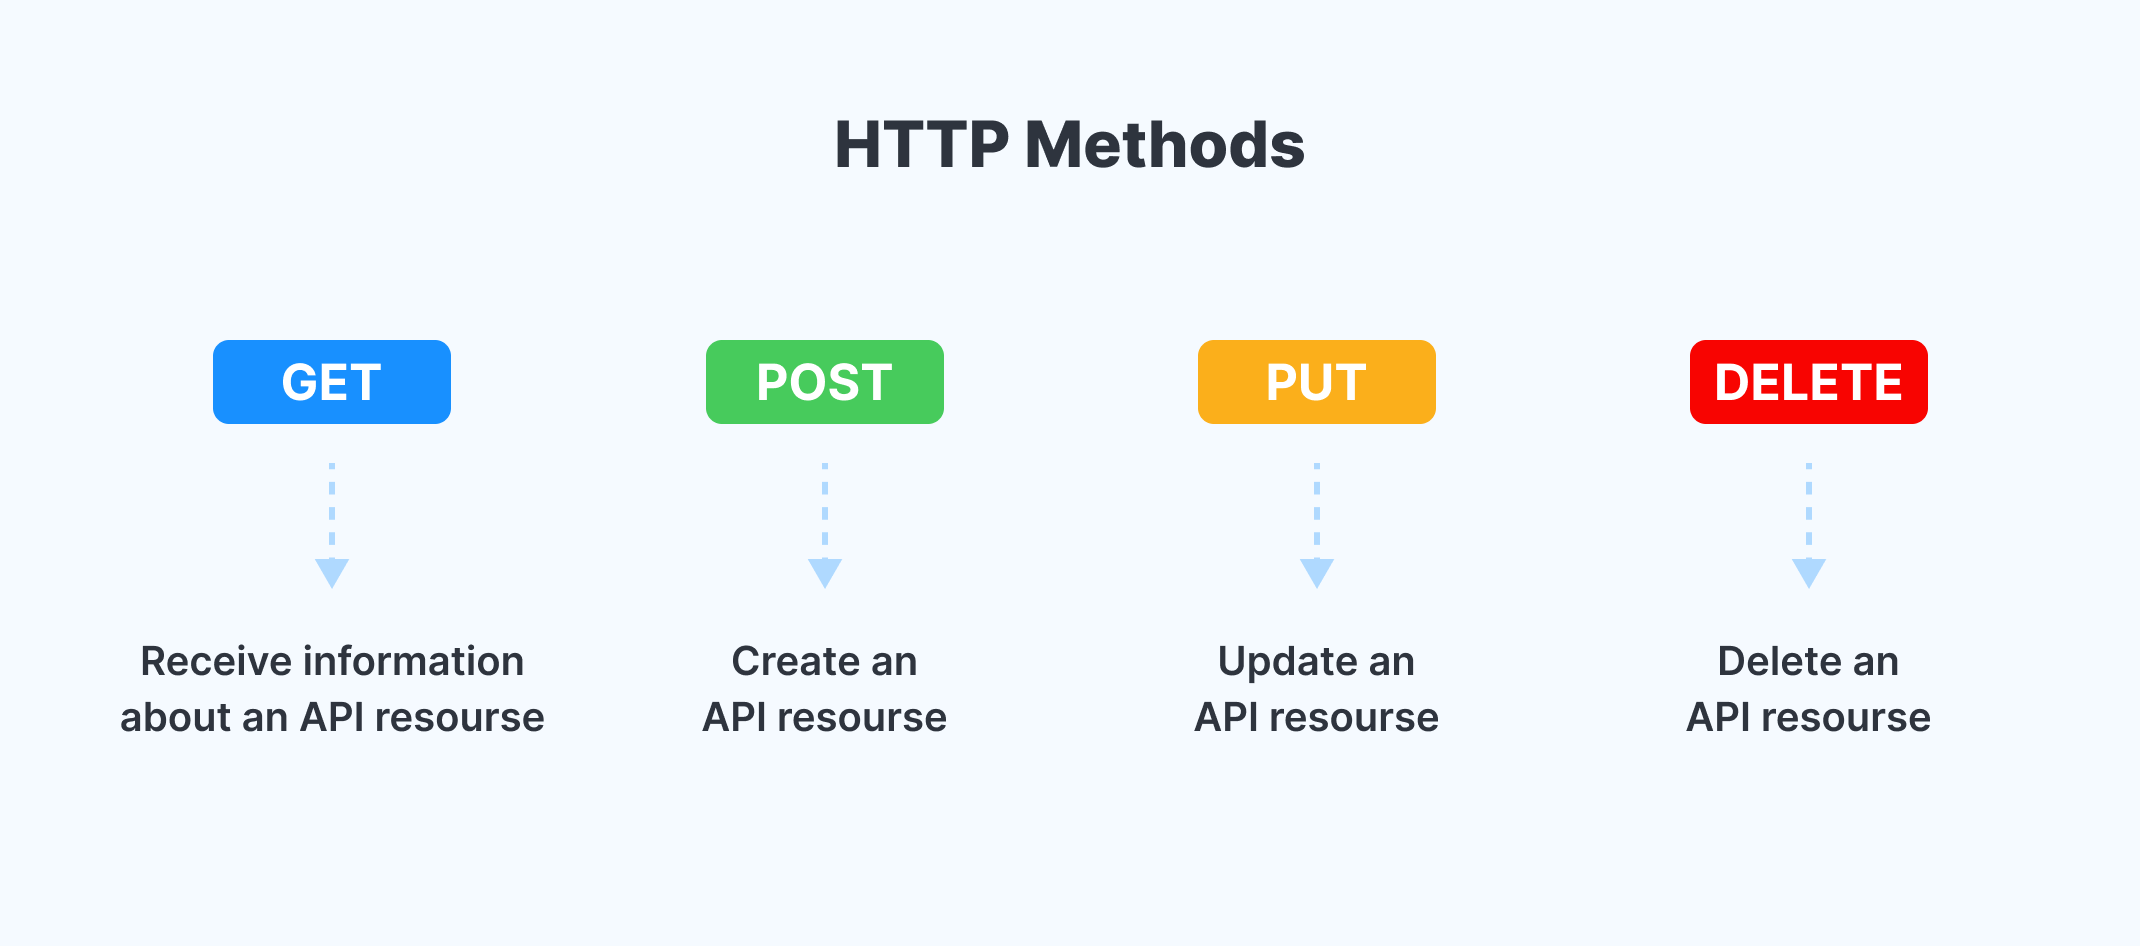
\includegraphics[width=0.8\textwidth]{pics/funktionsweiseRest.png}
  \centering
  \caption{HTTP-Methoden ~\cite{rest_api_model}}
\end{figure}

\subsubsection{HTTP-Response}
Ein HTTP-Response ist eine Antwort oder Meldung, die von Server zum Client gesendet wird. 
Ein HTTP-Response besteht aus einem Header mit optionalen Antwortparametern und einem Body, der
jedoch auch leer sein kann. 
Der Header enthält die Protokollversion, außerdem enthält er auch noch einen Statuscode und einer
Statusmeldung. Der Statuscode der Antwort teilt dem Client mit, ob
die gewünschte Operation vom Server ausgeführt werden konnte.
~\cite{http_response}

\subsubsection{TCP/IP-Protokoll}
Das TCP/IP-Protokoll ist eine Gruppe von Protokollen,
die die Grundlage für das Internet und andere Netzwerke bilden. 
Der Name TCP/IP setzt sich aus den beiden Protokollen Transmission Control Protocol (TCP) und 
Internetprotokoll (IP) zusammen. 
Wobei bei auch bei diesen Protokollen mehrere Protokollen zusammengefasst werden. 
Bei TCP/IP handelt es sich also um keine bestimmte Technik, sondern um eine Gruppierung von Protokollen.
\newline
\newline
Die Protokolle des TCP/IP-Models sind so standardisiert, dass es nicht von Wichtigkeit ist, 
welches Betriebssystem oder welches Gerät man für die Kommunikation über das Netzwerk verwendet.
~\cite{tcp_ip}

\section{Software-Testing}
\setauthor{Weissengruber Nina}
Software-Testing ist der Prozess, um die Funktionalität einer Softwareanwendung zu bewerten. 
Es dient zum Feststellen, ob die entwickelte Software die Anforderungen erfüllt oder nicht.
Es wird also das Ergebnis der Entwicklung getestet.
~\cite{software_testing}

\subsection{Testtechniken}
Man unterscheidet zwischen zwei Testtechniken
\subsubsection{Statische Testtechniken}
Statische Testtechniken dienen dem Überprüfen von Arbeitsergebnissen, ohne diese auf dem Rechner auszuführen.
\newline
Vorteile sind, dass es eine frühe Fehlererkennung gibt und Fehler direkt aufgedeckt werden.
Außerdem verringern sie die Anzahl von dynamischen Tests, welche aufwändiger und teuer sind.
\subsubsection{Dynamische Testtechniken}
Dynamische Testtechniken werden verwendet, um Fehler in der Software zu entdecken.
\newline
~\cite{software_testing_methoden}
Es gibt verschiedene dynamische Testtechniken. Die geläufigsten sind:
\begin{itemize}
  \item \textbf{"Black-Box-Testverfahren"}
  Dabei werden Testfälle nur anhand der Spezifikationen/Anforderungen erstellt, 
  ohne die innere Struktur zu berücksichtigen.
  ~\cite{black_box}
  \item \textbf{"White-Box-Testverfahren"}
  Berücksichtigt im Gegensatz zum Black-Box-Testverfahren das innere des Testobjekts,
  das heißt den Code.
  ~\cite{white_box}
  \item \textbf{"Erfahrungsbasierte Testverfahren"}
  Dabei werden Testfälle anhand von Erfahrungen, Wissen und Intuition der Tester erstellt.
  ~\cite{erfahrungsbasiertes_testen}
\end{itemize}

\subsection{Testarten}
Man unterscheidet zwischen verschiedenen Arten zu testen. Die Entscheidung, welcher Test verwendet werden
soll, hängt von dem Ziel ab, welches der Test erfüllen soll.
\subsubsection{Funktionale Tests}
Funktionale Tests konzentrieren sich auf Funktionen in der Anwendung und überprüfen, 
ob diese ihre Aufgabe richtig erfüllen.
\subsubsection{Nicht-funktionale Tests}
Nicht funktionale Tests überprüfen, wie gut die Anwendung im Ganzen funktioniert.
\begin{itemize}
  \item \textbf{"Performanz/ Effizienz"}
  wird durch Performanztests oder Lasttest geprüft.
  \item \textbf{"Zuverlässigkeit"}
  Zuverlässigkeitstest überprüfen, ob ein Testobjekt über einen bestimmten Zeitraum ein bestimmtes 
  Leistungsniveau unter bestimmten Bedingungen aufrechterhält.
  \item \textbf{"Benutzbarkeit/ Gebrauchstauglichkeit"}
  Benutzbarkeitstests prüfen, wie gut und einfach ein System für den Benutzer zu bedienen ist.
  \item \textbf{"Sicherheitstest"}
  überprüfen, ob System und Daten vor unerlaubten Zugriffen und externen Bedrohungen geschützt sind.
  \item \textbf{"Kompatibilität"}
  Interoperabilitätstest bewerten die Fähigkeit des Softwareprodukts.
  \item \textbf{"Wartbarkeit"}
  wird durch Reviews und werkzeuggeschützte statische Analyse geprüft.
  \item \textbf{"Übertragbarkeit"}
  wird durch Portabilitätstests getestet.
\end{itemize}
~\cite{software_testing_methoden}

\subsection{Unit Test}
Mithilfe von Unit Tests werden Komponenten des geschriebenen Codes überprüft. 
Der Code wird in einzelne Teile isoliert und diese Teile werden auf ihre Funktionalitäten überprüft.
\newline
\newline
Unit Tests sind nach den drei A's der Modultests aufgebaut.
\begin{itemize}
  \item \textbf{"Arrange (Anordnen)"}:
  Beim Arrange werden die Anforderungen definiert, die der Code erfüllen muss.
  \item \textbf{"Act (Handeln)"}:
  Beim Act wird der Test durchgeführt.
  \item \textbf{"Assert (Umsetzung)"}:
  Beim Assert werden die Ergebnisse überprüft. Wenn die Ergebnisse dem entsprechen, was erwartet
  wird, wird der Test validiert.
\end{itemize}
~\cite{unit_test}

\subsection{Smoke Test}
Smoke Test werden als Software-Probelauf bezeichnet. 
In einem kurzen Zeitraum soll die Funktionalität von neuen Funktionen und Anwendungen geprüft werden. 
Das Ziel von Smoke Tests ist es, Fehler zu finden, die später gravierende Probleme auslösen.
~\cite{smoke_test}

\subsection{Regressionstest}
Mithilfe von Regressionstests wird überprüft, ob Änderungen an der Anwendung oder andere dazugehörige
Softwarekomponenten Fehler herbeiführen und ob die Änderungen am Code die Funktionsweise beeinträchtigen 
oder stören.
\newline
\newline
Regressionstests können bei folgende Prozessen erforderlich sein:
\begin{itemize}
  \item beim Einführen von neuen Features
  \item beim Beheben eines Fehlers
  \item beim Refactoring zur Steigerung der Leistung
  \item beim Ändern der Hosting-Umgebung einer Anwendung
\end{itemize}

Regressionstests werden auf einer der folgenden Testebene durchgeführt:
\begin{itemize}
  \item Unit-Tests
  \item Integrationstests
  \item Systemtests
  \item Akzeptanztests
\end{itemize}
~\cite{regressionstests}

\subsection{Integrationstest}
Bei Integrationstests werden Units in Gruppen auf verschiedenste Weise kombiniert und getestet. 
Integrationstests können Probleme von Schnittstellen aufdecken. 
\newline
\newline
Es gibt 2 Methoden zur Durchführung von Integrationstest:
\begin{itemize}
  \item \textbf{"Bottom-up-Methode"}:
  Bottom-up Integrationstests beginnen mit Unit-Test, die gefolgt werden von Tests mit Kombinationen von Units.

  \item \textbf{"Top-down-Methode"}:
  Top-down Integrationstests beginnen damit, die Module höchster Ebene zu testen. Erst dann werden Module niedrigerer Ebenen getestet.

\end{itemize}
~\cite{integrationstests}

\subsection{Systemtests}
Bei Systemtests wird überprüft, wie die verschiedenen Komponenten im vollständigen System oder in der Anwedung
zusammenarbeiten.
\newline
Es gibt verschiedene Arten von Systemtests, welche unterschiedliche Komponenten testen:
\begin{itemize}
  \item \textbf{"Leistungstests:"}
  Geschwindigkeit, Stabilität, Reaktionszeiten
  \item \textbf{"Lasttests"}:
  Latenz, Anzahl der Benutzer
  \item \textbf{"Usability-Tests"}:
  Aufgabenerfolgsrate, Zeit bis Aufgaben erledigt sind
\end{itemize}
~\cite{systemtest}

\subsection{Testframeworks}
Testframeworks sind Richtlinien oder Regeln, die zum erstellen und entwerfen von Testfällen
verwendet werden.

~\cite{testframework}
